\documentclass{article}
\usepackage{amsmath, amssymb, graphicx, geometry, tikz, array, booktabs, enumitem, listings, xcolor, fancyhdr, float, subcaption, hyperref}

\title{Module 6: Linear Classification}
\author{Machine Learning Course}
\date{}

\begin{document}

\maketitle
\tableofcontents
\newpage

\section{Introduction to Linear Classification}

\subsection{Overview of Classification}
Classification is a fundamental task in machine learning where the goal is to assign discrete labels to data points. In binary classification, we aim to distinguish between two classes, typically labeled as $+1$ and $-1$. Linear classification is one of the simplest yet powerful approaches to this problem, using a linear decision boundary to separate the classes.

\subsection{Topics Covered}
This module explores several key aspects of linear classification:
\begin{enumerate}
    \item Linear decision boundaries for binary classification
    \item The Perceptron algorithm
    \item Maximizing the margin (Support Vector Machines)
    \item The soft-margin SVM for non-separable data
\end{enumerate}

\subsection{Applications}
Linear classification methods have numerous applications across various domains:
\begin{itemize}
    \item Text categorization (e.g., spam detection, sentiment analysis)
    \item Image recognition (e.g., simple object detection)
    \item Medical diagnosis (e.g., disease classification based on symptoms)
    \item Financial analysis (e.g., credit approval)
\end{itemize}

\section{Linear Decision Boundaries}

\subsection{Mathematical Formulation}
In binary classification, we have:
\begin{itemize}
    \item Data points $x \in \mathbb{R}^d$ (feature vectors in $d$-dimensional space)
    \item Labels $y \in \{-1, +1\}$ (binary class labels)
\end{itemize}

A linear classifier is defined by:
\begin{itemize}
    \item A weight vector $w \in \mathbb{R}^d$
    \item A bias term $b \in \mathbb{R}$
\end{itemize}

The decision boundary is the hyperplane defined by:
\begin{align}
w \cdot x + b = 0
\end{align}

\begin{figure}[h]
\centering
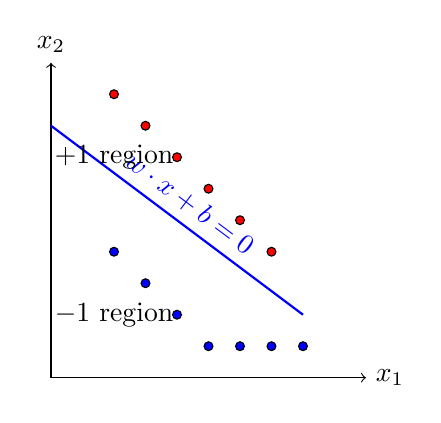
\begin{tikzpicture}[scale=0.8]
    % Coordinate axes
    \draw[->] (0,0) -- (5,0) node[right] {$x_1$};
    \draw[->] (0,0) -- (0,5) node[above] {$x_2$};
    
    % Decision boundary
    \draw[thick, blue] (0,4) -- (4,1) node[midway, above, sloped] {$w \cdot x + b = 0$};
    
    % Data points
    \foreach \x/\y in {1/4.5, 1.5/4, 2/3.5, 2.5/3, 3/2.5, 3.5/2}
        \draw[fill=red] (\x,\y) circle (2pt);
    
    \foreach \x/\y in {1/2, 1.5/1.5, 2/1, 2.5/0.5, 3/0.5, 3.5/0.5, 4/0.5}
        \draw[fill=blue] (\x,\y) circle (2pt);
    
    % Regions
    \node at (1,1) {$-1$ region};
    \node at (1,3.5) {$+1$ region};
\end{tikzpicture}
\caption{Example of a linear decision boundary separating two classes}
\end{figure}

\subsection{Making Predictions}
For a new data point $x$, the predicted label is:
\begin{align}
\hat{y} = \text{sign}(w \cdot x + b) = 
\begin{cases}
+1 & \text{if } w \cdot x + b > 0 \\
-1 & \text{if } w \cdot x + b < 0
\end{cases}
\end{align}

\subsection{Correctness Condition}
A linear classifier correctly classifies a point $(x, y)$ if and only if:
\begin{align}
y(w \cdot x + b) > 0
\end{align}

This elegant formulation combines both cases:
\begin{itemize}
    \item When $y = +1$, we need $w \cdot x + b > 0$
    \item When $y = -1$, we need $w \cdot x + b < 0$
\end{itemize}

\section{Loss Function for Classification}

\subsection{Defining the Loss}
To train a linear classifier, we need a loss function that quantifies how "wrong" our model is on a given example. A natural loss function for classification is:
\begin{align}
L(w, b; x, y) = 
\begin{cases}
0 & \text{if } y(w \cdot x + b) > 0 \text{ (correct classification)} \\
-y(w \cdot x + b) & \text{if } y(w \cdot x + b) \leq 0 \text{ (incorrect classification)}
\end{cases}
\end{align}

This loss function has several desirable properties:
\begin{itemize}
    \item Zero loss for correctly classified points
    \item Positive loss for incorrectly classified points
    \item The loss increases as the point gets further on the wrong side of the boundary
\end{itemize}

\subsection{Gradient of the Loss}
For stochastic gradient descent, we need the gradient of the loss function:
\begin{align}
\nabla_w L(w, b; x, y) &= 
\begin{cases}
0 & \text{if } y(w \cdot x + b) > 0 \\
-yx & \text{if } y(w \cdot x + b) \leq 0
\end{cases} \\
\frac{\partial L}{\partial b}(w, b; x, y) &= 
\begin{cases}
0 & \text{if } y(w \cdot x + b) > 0 \\
-y & \text{if } y(w \cdot x + b) \leq 0
\end{cases}
\end{align}

\section{The Perceptron Algorithm}

\subsection{Algorithm Description}
The Perceptron is a simple yet powerful algorithm for learning linear classifiers. It iteratively updates the model parameters based on misclassified points.

\fbox{
\begin{minipage}{\dimexpr\textwidth-2\fboxsep-2\fboxrule\relax}
\textbf{The Perceptron Algorithm}
\begin{enumerate}
    \item Initialize $w = 0$ and $b = 0$
    \item Repeat until convergence:
    \begin{enumerate}
        \item For each training example $(x, y)$:
        \begin{enumerate}
            \item If $y(w \cdot x + b) \leq 0$ (point is misclassified):
            \begin{enumerate}
                \item $w = w + yx$
                \item $b = b + y$
            \end{enumerate}
        \end{enumerate}
    \end{enumerate}
\end{enumerate}
\end{minipage}
}

\subsection{Connection to Stochastic Gradient Descent}
The Perceptron update rule can be derived from stochastic gradient descent on the loss function defined earlier:
\begin{align}
w &= w - \eta \nabla_w L(w, b; x, y) \\
b &= b - \eta \frac{\partial L}{\partial b}(w, b; x, y)
\end{align}

With learning rate $\eta = 1$ and for misclassified points where $y(w \cdot x + b) \leq 0$:
\begin{align}
w &= w - (-yx) = w + yx \\
b &= b - (-y) = b + y
\end{align}

\subsection{The Perceptron in Action}
The Perceptron algorithm has been shown to work well on linearly separable data. For example, on a dataset with 85 linearly separable points, the Perceptron successfully finds a decision boundary that correctly classifies all points.

\begin{figure}[h]
\centering
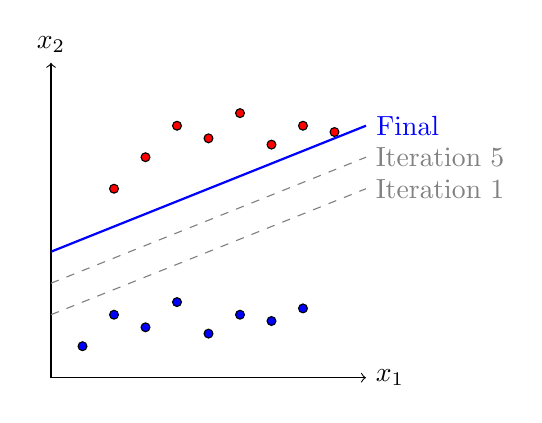
\begin{tikzpicture}[scale=0.8]
    % Coordinate axes
    \draw[->] (0,0) -- (5,0) node[right] {$x_1$};
    \draw[->] (0,0) -- (0,5) node[above] {$x_2$};
    
    % Data points (simplified representation)
    \foreach \x/\y in {0.5/0.5, 1/1, 1.5/0.8, 2/1.2, 2.5/0.7, 3/1, 3.5/0.9, 4/1.1}
        \draw[fill=blue] (\x,\y) circle (2pt);
    
    \foreach \x/\y in {1/3, 1.5/3.5, 2/4, 2.5/3.8, 3/4.2, 3.5/3.7, 4/4, 4.5/3.9}
        \draw[fill=red] (\x,\y) circle (2pt);
    
    % Decision boundaries at different iterations
    \draw[dashed, gray] (0,1) -- (5,3) node[right] {Iteration 1};
    \draw[dashed, gray] (0,1.5) -- (5,3.5) node[right] {Iteration 5};
    \draw[thick, blue] (0,2) -- (5,4) node[right] {Final};
\end{tikzpicture}
\caption{Illustration of Perceptron convergence on linearly separable data. The decision boundary evolves over iterations until it perfectly separates the classes.}
\end{figure}

\subsection{Perceptron Convergence Theorem}
A fundamental result for the Perceptron algorithm:

\fbox{
\begin{minipage}{\dimexpr\textwidth-2\fboxsep-2\fboxrule\relax}
\textbf{Perceptron Convergence Theorem}

If the training data is linearly separable, then:
\begin{itemize}
    \item The Perceptron algorithm will find a linear classifier with zero training error
    \item It will converge within a finite number of steps
\end{itemize}
\end{minipage}
}

However, the Perceptron algorithm has limitations:
\begin{itemize}
    \item It only works for linearly separable data
    \item It may find any linear separator that works, not necessarily the "best" one
    \item The solution depends on the order of processing the training examples
\end{itemize}

This raises an important question: Among all possible linear separators, which one should we choose?

\section{The Hard-Margin Support Vector Machine}

\subsection{The Margin Concept}
The margin of a linear classifier is the distance from the decision boundary to the nearest training point. A classifier with a large margin is likely to generalize better to unseen data.

\begin{figure}[h]
\centering
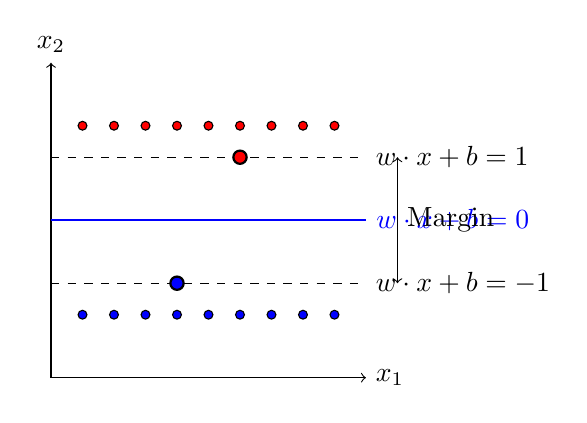
\begin{tikzpicture}[scale=0.8]
    % Coordinate axes
    \draw[->] (0,0) -- (5,0) node[right] {$x_1$};
    \draw[->] (0,0) -- (0,5) node[above] {$x_2$};
    
    % Decision boundary
    \draw[thick, blue] (0,2.5) -- (5,2.5) node[right] {$w \cdot x + b = 0$};
    
    % Margin boundaries
    \draw[dashed] (0,1.5) -- (5,1.5) node[right] {$w \cdot x + b = -1$};
    \draw[dashed] (0,3.5) -- (5,3.5) node[right] {$w \cdot x + b = 1$};
    
    % Margin
    \draw[<->] (5.5,1.5) -- (5.5,3.5) node[midway, right] {Margin};
    
    % Data points
    \foreach \x in {0.5,1,...,4.5}
        \draw[fill=blue] (\x,1) circle (2pt);
    
    \foreach \x in {0.5,1,...,4.5}
        \draw[fill=red] (\x,4) circle (2pt);
    
    % Support vectors
    \draw[fill=blue, thick] (2,1.5) circle (3pt);
    \draw[fill=red, thick] (3,3.5) circle (3pt);
\end{tikzpicture}
\caption{Illustration of the margin in a linearly separable dataset. The support vectors (highlighted) lie exactly on the margin boundaries.}
\end{figure}

\subsection{The Learning Problem}
Given training data $\{(x^{(i)}, y^{(i)}): i=1,\ldots,n\} \subset \mathbb{R}^d \times \{-1, +1\}$, we want to find $w \in \mathbb{R}^d$ and $b \in \mathbb{R}$ such that:
\begin{align}
y^{(i)}(w \cdot x^{(i)} + b) > 0 \quad \text{for all } i=1,\ldots,n
\end{align}

By scaling $w$ and $b$, we can equivalently require:
\begin{align}
y^{(i)}(w \cdot x^{(i)} + b) \geq 1 \quad \text{for all } i=1,\ldots,n
\end{align}

This formulation ensures that all points are not only correctly classified but also at least a certain distance from the decision boundary.

\subsection{Maximizing the Margin}
The margin $\gamma$ of a linear classifier is the distance from the decision boundary to the nearest training point. For a linear classifier with $\|w\| = 1$, this distance is given by $|w \cdot x + b|$.

With our constraint $y^{(i)}(w \cdot x^{(i)} + b) \geq 1$, the margin is $\gamma = 1/\|w\|$.

Therefore, maximizing the margin is equivalent to minimizing $\|w\|$, or equivalently, minimizing $\|w\|^2$ (which is differentiable everywhere).

\subsection{The Optimization Problem}
The hard-margin SVM optimization problem is:

\fbox{
\begin{minipage}{\dimexpr\textwidth-2\fboxsep-2\fboxrule\relax}
\textbf{Hard-Margin SVM Optimization Problem}

\begin{align}
\min_{w \in \mathbb{R}^d, b \in \mathbb{R}} & \|w\|^2 \\
\text{subject to: } & y^{(i)}(w \cdot x^{(i)} + b) \geq 1 \quad \text{for all } i = 1, 2, \ldots, n
\end{align}
\end{minipage}
}

This is a convex quadratic optimization problem with linear constraints, which means:
\begin{itemize}
    \item It has a unique global minimum
    \item It can be solved efficiently using standard optimization techniques
    \item Duality theory provides insights into the structure of the solution
\end{itemize}

\subsection{Support Vectors}
The solution to the SVM optimization problem has an interesting property: most training points have no influence on the decision boundary. The only points that matter are those that lie exactly on the margin, i.e., points for which $y^{(i)}(w \cdot x^{(i)} + b) = 1$. These points are called support vectors.

The optimal weight vector can be expressed as a linear combination of the support vectors:
\begin{align}
w = \sum_{i=1}^{n} \alpha_i y^{(i)} x^{(i)}
\end{align}
where $\alpha_i \geq 0$ are Lagrange multipliers that are non-zero only for support vectors.

\begin{figure}[h]
\centering
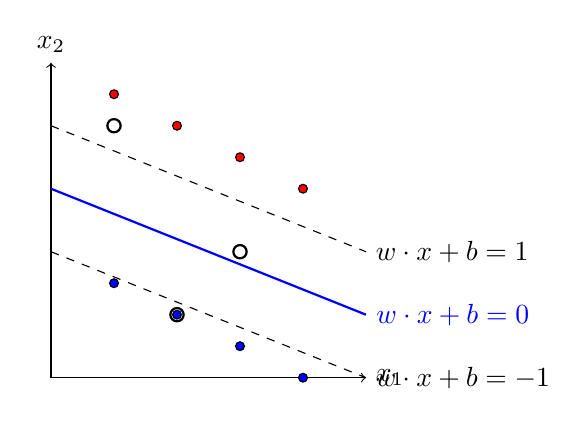
\begin{tikzpicture}[scale=0.8]
    % Coordinate axes
    \draw[->] (0,0) -- (5,0) node[right] {$x_1$};
    \draw[->] (0,0) -- (0,5) node[above] {$x_2$};
    
    % Decision boundary
    \draw[thick, blue] (0,3) -- (5,1) node[right] {$w \cdot x + b = 0$};
    
    % Margin boundaries
    \draw[dashed] (0,4) -- (5,2) node[right] {$w \cdot x + b = 1$};
    \draw[dashed] (0,2) -- (5,0) node[right] {$w \cdot x + b = -1$};
    
    % Data points
    \foreach \x/\y in {1/4.5, 2/4, 3/3.5, 4/3}
        \draw[fill=red] (\x,\y) circle (2pt);
    
    \foreach \x/\y in {1/1.5, 2/1, 3/0.5, 4/0}
        \draw[fill=blue] (\x,\y) circle (2pt);
    
    % Support vectors
    \draw[thick] (1,4) circle (3pt);
    \draw[thick] (3,2) circle (3pt);
    \draw[thick] (2,1) circle (3pt);
\end{tikzpicture}
\caption{Support vectors are the points that lie exactly on the margin boundaries. The decision boundary is determined entirely by these points.}
\end{figure}

\section{Example: Iris Dataset}

\subsection{Dataset Description}
The Iris dataset is a classic dataset in machine learning, collected by the botanist Edgar Anderson and made famous by the statistician Ronald Fisher. It contains measurements of 150 iris flowers from three different species:

\begin{itemize}
    \item Iris setosa
    \item Iris versicolor
    \item Iris virginica
\end{itemize}

For each flower, four measurements were taken:
\begin{itemize}
    \item Sepal length
    \item Sepal width
    \item Petal length
    \item Petal width
\end{itemize}

\subsection{Binary Classification Example}
For simplicity, we can consider a binary classification problem using only two of the species (setosa and versicolor) and two of the features (sepal width and petal width).

\begin{figure}[h]
\centering
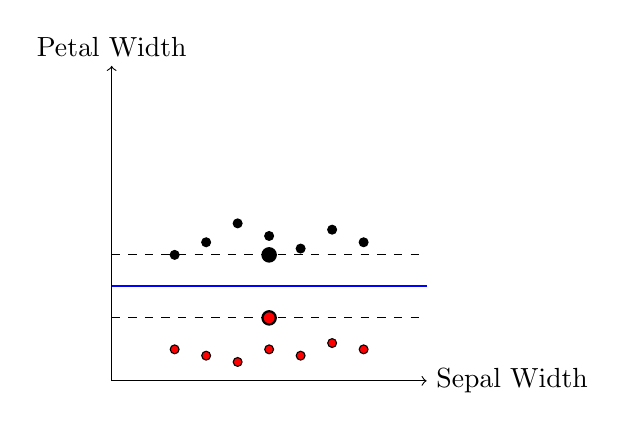
\begin{tikzpicture}[scale=0.8]
    % Coordinate axes
    \draw[->] (0,0) -- (5,0) node[right] {Sepal Width};
    \draw[->] (0,0) -- (0,5) node[above] {Petal Width};
    
    % Setosa (red circles)
    \foreach \x/\y in {1/0.5, 1.5/0.4, 2/0.3, 2.5/0.5, 3/0.4, 3.5/0.6, 4/0.5}
        \draw[fill=red] (\x,\y) circle (2pt);
    
    % Versicolor (black triangles)
    \foreach \x/\y in {1/2, 1.5/2.2, 2/2.5, 2.5/2.3, 3/2.1, 3.5/2.4, 4/2.2}
        \draw[fill=black] (\x,\y) circle (2pt);
    
    % Decision boundary
    \draw[thick, blue] (0,1.5) -- (5,1.5);
    
    % Margin boundaries
    \draw[dashed] (0,1) -- (5,1);
    \draw[dashed] (0,2) -- (5,2);
    
    % Support vectors
    \draw[fill=red, thick] (2.5,1) circle (3pt);
    \draw[fill=black, thick] (2.5,2) circle (3pt);
\end{tikzpicture}
\caption{SVM classification of Iris setosa (red circles) and Iris versicolor (black triangles) using sepal width and petal width features.}
\end{figure}

In this example, the data is linearly separable, and the SVM finds the maximum-margin linear classifier. The support vectors are the points that lie exactly on the margin boundaries.

\section{The Soft-Margin SVM}

\subsection{Handling Non-linearly Separable Data}
The hard-margin SVM assumes that the data is linearly separable. However, in real-world scenarios, data is often not perfectly separable due to noise or outliers. To handle such cases, we can use a soft-margin SVM, which allows for some misclassifications.

\subsection{Slack Variables}
We introduce slack variables $\xi_i \geq 0$ for each training point, which measure the degree of misclassification:

\begin{align}
y^{(i)}(w \cdot x^{(i)} + b) \geq 1 - \xi_i \quad \text{for all } i = 1, 2, \ldots, n
\end{align}

The interpretation of $\xi_i$ is:
\begin{itemize}
    \item $\xi_i = 0$: The point is correctly classified and on or beyond the margin
    \item $0 < \xi_i \leq 1$: The point is correctly classified but within the margin
    \item $\xi_i > 1$: The point is misclassified
\end{itemize}

\subsection{The Optimization Problem}
The soft-margin SVM optimization problem is:

\fbox{
\begin{minipage}{\dimexpr\textwidth-2\fboxsep-2\fboxrule\relax}
\textbf{Soft-Margin SVM Optimization Problem}

\begin{align}
\min_{w \in \mathbb{R}^d, b \in \mathbb{R}, \xi \in \mathbb{R}^n} & \|w\|^2 + C \sum_{i=1}^{n} \xi_i \\
\text{subject to: } & y^{(i)}(w \cdot x^{(i)} + b) \geq 1 - \xi_i \quad \text{for all } i = 1, 2, \ldots, n \\
& \xi_i \geq 0 \quad \text{for all } i = 1, 2, \ldots, n
\end{align}
\end{minipage}
}

The parameter $C > 0$ controls the trade-off between maximizing the margin and minimizing the classification error. A larger $C$ places more emphasis on correctly classifying all training points, while a smaller $C$ places more emphasis on maximizing the margin.

\begin{figure}[h]
\centering
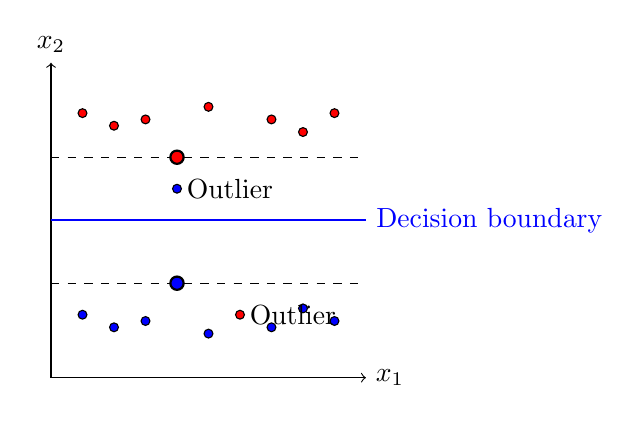
\begin{tikzpicture}[scale=0.8]
    % Coordinate axes
    \draw[->] (0,0) -- (5,0) node[right] {$x_1$};
    \draw[->] (0,0) -- (0,5) node[above] {$x_2$};
    
    % Decision boundary
    \draw[thick, blue] (0,2.5) -- (5,2.5) node[right] {Decision boundary};
    
    % Margin boundaries
    \draw[dashed] (0,1.5) -- (5,1.5);
    \draw[dashed] (0,3.5) -- (5,3.5);
    
    % Data points
    \foreach \x/\y in {0.5/1, 1/0.8, 1.5/0.9, 2.5/0.7, 3.5/0.8, 4/1.1, 4.5/0.9}
        \draw[fill=blue] (\x,\y) circle (2pt);
    
    \foreach \x/\y in {0.5/4.2, 1/4, 1.5/4.1, 2.5/4.3, 3.5/4.1, 4/3.9, 4.5/4.2}
        \draw[fill=red] (\x,\y) circle (2pt);
    
    % Outliers
    \draw[fill=blue] (2,3) circle (2pt) node[right] {Outlier};
    \draw[fill=red] (3,1) circle (2pt) node[right] {Outlier};
    
    % Support vectors
    \draw[fill=blue, thick] (2,1.5) circle (3pt);
    \draw[fill=red, thick] (2,3.5) circle (3pt);
\end{tikzpicture}
\caption{Soft-margin SVM allows for some misclassifications to handle outliers or non-linearly separable data.}
\end{figure}

\section{Parameter Selection for SVMs}

\subsection{The Role of Parameter $C$}
The parameter $C$ in the soft-margin SVM formulation controls the trade-off between maximizing the margin and minimizing the classification error:

\begin{itemize}
    \item Small $C$: Places more emphasis on maximizing the margin, even if it means allowing more training errors
    \item Large $C$: Places more emphasis on minimizing training errors, potentially at the cost of a smaller margin
\end{itemize}

\begin{figure}[h]
\centering
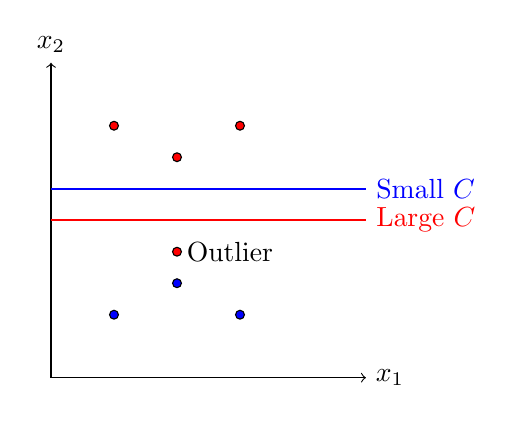
\begin{tikzpicture}[scale=0.8]
    % Coordinate axes
    \draw[->] (0,0) -- (5,0) node[right] {$x_1$};
    \draw[->] (0,0) -- (0,5) node[above] {$x_2$};
    
    % Data points
    \draw[fill=red] (1,4) circle (2pt);
    \draw[fill=red] (2,3.5) circle (2pt);
    \draw[fill=red] (3,4) circle (2pt);
    \draw[fill=blue] (1,1) circle (2pt);
    \draw[fill=blue] (2,1.5) circle (2pt);
    \draw[fill=blue] (3,1) circle (2pt);
    
    % Outlier
    \draw[fill=red] (2,2) circle (2pt) node[right] {Outlier};
    
    % Decision boundaries
    \draw[thick, blue] (0,3) -- (5,3) node[right] {Small $C$};
    \draw[thick, red] (0,2.5) -- (5,2.5) node[right] {Large $C$};
\end{tikzpicture}
\caption{Effect of parameter $C$ on the decision boundary. A small $C$ (blue line) allows the outlier to be misclassified to maintain a larger margin. A large $C$ (red line) adjusts the boundary to correctly classify the outlier, resulting in a smaller margin.}
\end{figure}

\subsection{Practical Implications}
The choice of $C$ has significant practical implications:

\begin{itemize}
    \item \textbf{Overfitting vs. Underfitting}: Large $C$ values can lead to overfitting, while small $C$ values might result in underfitting
    \item \textbf{Number of Support Vectors}: Larger $C$ values typically result in fewer support vectors
    \item \textbf{Generalization Performance}: The optimal $C$ value balances training accuracy and generalization to unseen data
\end{itemize}

\section{Sentiment Analysis Example}

\subsection{Dataset Description}
To illustrate the importance of parameter selection, we'll examine a sentiment analysis dataset:

\begin{itemize}
    \item \textbf{Source}: Reviews from Amazon, Yelp, and IMDB
    \item \textbf{Labels}: Binary classification (positive or negative sentiment)
    \item \textbf{Representation}: Bag-of-words with a vocabulary of 4500 words
    \item \textbf{Size}: 2500 training sentences, 500 test sentences
\end{itemize}

\subsection{Example Sentences}
The dataset contains sentences like:

\begin{itemize}
    \item "Needless to say, I wasted my money." (Negative)
    \item "He was very impressed when going from the original battery to the extended battery." (Positive)
    \item "I have to jiggle the plug to get it to line up right to get decent volume." (Negative)
    \item "Will order from them again!" (Positive)
\end{itemize}

\subsection{Feature Representation}
The bag-of-words representation transforms each sentence into a high-dimensional vector:

\begin{itemize}
    \item Each dimension corresponds to a word in the vocabulary
    \item The value in each dimension represents the presence or frequency of the word in the sentence
    \item This creates a sparse vector representation (most entries are zero)
\end{itemize}

\begin{figure}[h]
\centering
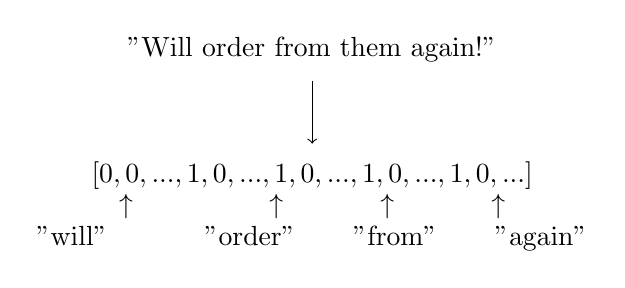
\begin{tikzpicture}[scale=0.8]
    % Sentence
    \node[align=left] at (0,4) {"Will order from them again!"};
    
    % Arrow
    \draw[->] (0,3.5) -- (0,2.5);
    
    % Vector representation
    \node[align=left] at (0,2) {$[0, 0, ..., 1, 0, ..., 1, 0, ..., 1, 0, ..., 1, 0, ...]$};
    \node[align=left] at (0,1.5) {$\uparrow$ \hspace{1.5cm} $\uparrow$ \hspace{1cm} $\uparrow$ \hspace{1cm} $\uparrow$};
    \node[align=left] at (0,1) {"will" \hspace{1cm} "order" \hspace{0.5cm} "from" \hspace{0.5cm} "again"};
\end{tikzpicture}
\caption{Bag-of-words representation of a sentence. Each word in the vocabulary corresponds to a dimension in the feature vector.}
\end{figure}

\section{Experimental Results with Different $C$ Values}

\subsection{Performance Metrics}
For each value of $C$, we measure three key metrics:

\begin{itemize}
    \item \textbf{Training error}: Percentage of misclassified training examples
    \item \textbf{Test error}: Percentage of misclassified test examples
    \item \textbf{Number of support vectors}: Points that influence the decision boundary
\end{itemize}

\subsection{Results Table}
\begin{table}[h]
\centering
\begin{tabular}{|c|c|c|c|}
\hline
\textbf{C} & \textbf{Training Error (\%)} & \textbf{Test Error (\%)} & \textbf{\# Support Vectors} \\
\hline
0.01 & 23.72 & 28.4 & 2294 \\
0.1 & 7.88 & 18.4 & 1766 \\
1 & 1.12 & 16.8 & 1306 \\
10 & 0.16 & 19.4 & 1105 \\
100 & 0.08 & 19.4 & 1035 \\
1000 & 0.08 & 19.4 & 950 \\
\hline
\end{tabular}
\caption{Performance metrics for different values of parameter $C$ on the sentiment analysis dataset}
\end{table}

\subsection{Analysis of Results}
Several important trends can be observed from the experimental results:

\begin{enumerate}
    \item \textbf{Training Error}: Decreases monotonically as $C$ increases
    \begin{itemize}
        \item At $C = 0.01$: High training error (23.72\%)
        \item At $C = 1000$: Near-zero training error (0.08\%)
    \end{itemize}
    
    \item \textbf{Test Error}: Initially decreases as $C$ increases, then increases
    \begin{itemize}
        \item At $C = 0.01$: High test error (28.4\%)
        \item At $C = 1$: Lowest test error (16.8\%)
        \item At $C \geq 10$: Test error increases to 19.4\%
    \end{itemize}
    
    \item \textbf{Number of Support Vectors}: Decreases as $C$ increases
    \begin{itemize}
        \item At $C = 0.01$: Many support vectors (2294)
        \item At $C = 1000$: Fewer support vectors (950)
    \end{itemize}
\end{enumerate}

\begin{figure}[h]
\centering
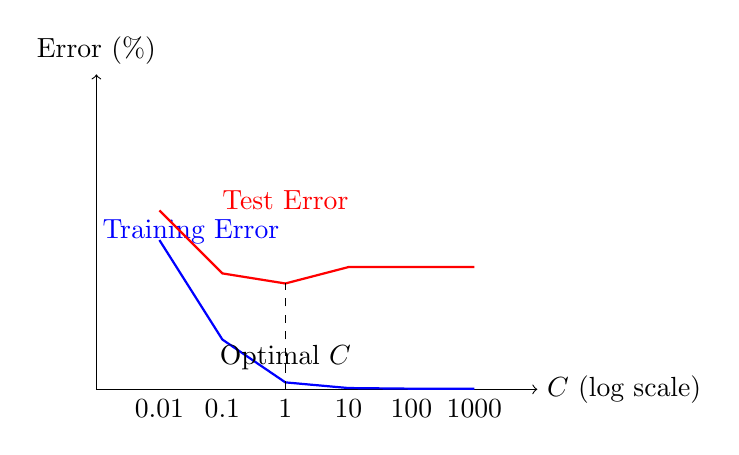
\begin{tikzpicture}[scale=0.8]
    % Coordinate axes
    \draw[->] (0,0) -- (7,0) node[right] {$C$ (log scale)};
    \draw[->] (0,0) -- (0,5) node[above] {Error (\%)};
    
    % X-axis labels
    \node at (1,-0.3) {0.01};
    \node at (2,-0.3) {0.1};
    \node at (3,-0.3) {1};
    \node at (4,-0.3) {10};
    \node at (5,-0.3) {100};
    \node at (6,-0.3) {1000};
    
    % Training error
    \draw[thick, blue] (1,2.37) -- (2,0.79) -- (3,0.11) -- (4,0.02) -- (5,0.01) -- (6,0.01);
    \node[blue] at (1.5,2.5) {Training Error};
    
    % Test error
    \draw[thick, red] (1,2.84) -- (2,1.84) -- (3,1.68) -- (4,1.94) -- (5,1.94) -- (6,1.94);
    \node[red] at (3,3) {Test Error};
    
    % Optimal C
    \draw[dashed] (3,0) -- (3,1.68);
    \node at (3,0.5) {Optimal $C$};
\end{tikzpicture}
\caption{Training and test error as a function of parameter $C$ (log scale). The optimal $C$ value minimizes the test error.}
\end{figure}

\section{Cross-Validation for Parameter Tuning}

\subsection{The Cross-Validation Procedure}
To find the optimal value of $C$, we can use cross-validation:

\begin{enumerate}
    \item Divide the training data into $k$ equal folds (e.g., $k = 5$)
    \item For each value of $C$:
    \begin{enumerate}
        \item For each fold $i$ (from 1 to $k$):
        \begin{enumerate}
            \item Train an SVM on all folds except fold $i$
            \item Evaluate the model on fold $i$
        \end{enumerate}
        \item Calculate the average error across all $k$ folds
    \end{enumerate}
    \item Select the $C$ value with the lowest average error
\end{enumerate}

\begin{figure}[h]
\centering
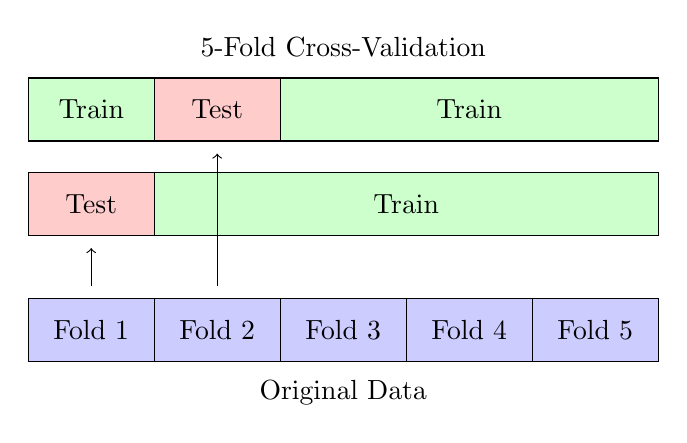
\begin{tikzpicture}[scale=0.8]
    % Data folds
    \draw[fill=blue!20] (0,0) rectangle (2,1) node[pos=0.5] {Fold 1};
    \draw[fill=blue!20] (2,0) rectangle (4,1) node[pos=0.5] {Fold 2};
    \draw[fill=blue!20] (4,0) rectangle (6,1) node[pos=0.5] {Fold 3};
    \draw[fill=blue!20] (6,0) rectangle (8,1) node[pos=0.5] {Fold 4};
    \draw[fill=blue!20] (8,0) rectangle (10,1) node[pos=0.5] {Fold 5};
    
    % Iteration 1
    \draw[fill=red!20] (0,2) rectangle (2,3) node[pos=0.5] {Test};
    \draw[fill=green!20] (2,2) rectangle (10,3) node[pos=0.5] {Train};
    
    % Iteration 2
    \draw[fill=green!20] (0,3.5) rectangle (2,4.5) node[pos=0.5] {Train};
    \draw[fill=red!20] (2,3.5) rectangle (4,4.5) node[pos=0.5] {Test};
    \draw[fill=green!20] (4,3.5) rectangle (10,4.5) node[pos=0.5] {Train};
    
    % Arrows
    \draw[->] (1,1.2) -- (1,1.8);
    \draw[->] (3,1.2) -- (3,3.3);
    
    % Labels
    \node at (5,-0.5) {Original Data};
    \node at (5,5) {5-Fold Cross-Validation};
\end{tikzpicture}
\caption{Illustration of 5-fold cross-validation. The data is divided into 5 folds, and each fold serves as the test set once while the remaining folds form the training set.}
\end{figure}

\subsection{Cross-Validation Results}
For the sentiment analysis dataset, 5-fold cross-validation was performed to select the optimal $C$ value:

\begin{itemize}
    \item The optimal value was found to be $C = 0.32$
    \item With this value, the test error was 15.6\%
\end{itemize}

This is better than any of the individual $C$ values tested in the previous experiment, highlighting the importance of proper parameter tuning.

\section{Interpreting the Trade-offs}

\subsection{Bias-Variance Trade-off}
The results illustrate the classic bias-variance trade-off in machine learning:

\begin{itemize}
    \item \textbf{Small $C$ values} (e.g., $C = 0.01$):
    \begin{itemize}
        \item High bias (underfitting)
        \item Simple model with large margin
        \item High training and test error
    \end{itemize}
    
    \item \textbf{Large $C$ values} (e.g., $C = 1000$):
    \begin{itemize}
        \item High variance (overfitting)
        \item Complex model with small margin
        \item Low training error but higher test error
    \end{itemize}
    
    \item \textbf{Optimal $C$ value} (e.g., $C = 0.32$ from cross-validation):
    \begin{itemize}
        \item Balances bias and variance
        \item Moderate margin size
        \item Best generalization performance
    \end{itemize}
\end{itemize}

\subsection{Margin vs. Classification Accuracy}
The parameter $C$ controls the trade-off between margin size and classification accuracy:

\begin{itemize}
    \item \textbf{Small $C$}: Prioritizes larger margins at the expense of training accuracy
    \item \textbf{Large $C$}: Prioritizes training accuracy at the expense of margin size
\end{itemize}

\subsection{Model Complexity}
The number of support vectors is an indicator of model complexity:

\begin{itemize}
    \item More support vectors generally mean a more complex model
    \item As $C$ increases, the number of support vectors decreases
    \item However, too few support vectors might indicate overfitting to the training data
\end{itemize}

\section{Practical Considerations}

\subsection{Feature Scaling}
SVMs are sensitive to the scale of the features. It's generally recommended to scale the features before training an SVM:

\begin{itemize}
    \item \textbf{Standardization}: $x' = \frac{x - \mu}{\sigma}$
    \item \textbf{Min-max scaling}: $x' = \frac{x - \min(x)}{\max(x) - \min(x)}$
\end{itemize}

\subsection{Handling Large Datasets}
Standard SVM implementations have time complexity $O(n^2)$ to $O(n^3)$, where $n$ is the number of training examples. This can be prohibitive for large datasets. Several approaches exist for scaling SVMs to large datasets:

\begin{itemize}
    \item \textbf{Chunking}: Solve the optimization problem in smaller chunks
    \item \textbf{Sequential Minimal Optimization (SMO)}: Optimize two Lagrange multipliers at a time
    \item \textbf{Stochastic gradient descent}: Approximate the SVM solution using SGD
    \item \textbf{Linear SVMs}: For linear kernels, specialized algorithms like LIBLINEAR can scale to millions of examples
\end{itemize}

\subsection{Kernel Selection}
While linear SVMs are effective for many high-dimensional problems (like text classification), non-linear kernels can be useful for other types of data:

\begin{itemize}
    \item \textbf{Linear kernel}: $K(x, z) = x \cdot z$
    \item \textbf{Polynomial kernel}: $K(x, z) = (x \cdot z + c)^d$
    \item \textbf{Radial Basis Function (RBF) kernel}: $K(x, z) = \exp(-\gamma \|x - z\|^2)$
    \item \textbf{Sigmoid kernel}: $K(x, z) = \tanh(\alpha x \cdot z + c)$
\end{itemize}

\subsection{Multi-class Classification}
SVMs are inherently binary classifiers, but they can be extended to multi-class problems using several strategies:

\begin{itemize}
    \item \textbf{One-vs-Rest}: Train $k$ binary SVMs, each separating one class from the rest
    \item \textbf{One-vs-One}: Train $\binom{k}{2}$ binary SVMs, one for each pair of classes
    \item \textbf{Direct Multi-class Formulation}: Extend the SVM optimization problem to directly handle multiple classes
\end{itemize}

\section{Summary and Key Takeaways}

\subsection{Linear Classification Approaches}
We've explored several approaches to linear classification:

\begin{itemize}
    \item \textbf{Perceptron}: A simple, iterative algorithm that finds any linear separator for linearly separable data
    \item \textbf{Hard-margin SVM}: Finds the maximum-margin linear separator for linearly separable data
    \item \textbf{Soft-margin SVM}: Extends the hard-margin SVM to handle non-linearly separable data by allowing some misclassifications
\end{itemize}

\subsection{The Importance of Parameter Tuning}
The soft-margin SVM parameter $C$ controls the trade-off between margin size and classification accuracy:

\begin{itemize}
    \item Small $C$ values prioritize larger margins, potentially allowing more training errors
    \item Large $C$ values prioritize minimizing training errors, potentially at the cost of smaller margins
    \item The optimal $C$ value balances these trade-offs to achieve the best generalization performance
    \item Cross-validation is an effective method for selecting the optimal $C$ value
\end{itemize}

\subsection{Practical Guidelines}
Based on our exploration, here are some practical guidelines for using linear classifiers:

\begin{itemize}
    \item \textbf{Start with a linear SVM}: For many problems, especially high-dimensional ones like text classification, a linear SVM is a good baseline
    \item \textbf{Use cross-validation for parameter tuning}: Test a range of $C$ values (e.g., $10^{-2}$ to $10^3$) and select the one with the best validation performance
    \item \textbf{Monitor both training and test performance}: This helps identify underfitting or overfitting
    \item \textbf{Consider the number of support vectors}: Too many might indicate underfitting, while too few might indicate overfitting
    \item \textbf{Scale features appropriately}: SVMs are sensitive to the scale of the features
    \item \textbf{For non-linear problems}: Consider using kernel SVMs or other non-linear classifiers
\end{itemize}

\subsection{Future Directions}
Linear classification continues to be an active area of research and development:

\begin{itemize}
    \item \textbf{Scalable algorithms}: Developing more efficient algorithms for large-scale linear classification
    \item \textbf{Online learning}: Adapting linear classifiers for streaming data
    \item \textbf{Deep learning}: Combining linear classifiers with deep neural networks
    \item \textbf{Interpretability}: Enhancing the interpretability of linear classifiers for complex domains
\end{itemize}

\end{document}